\documentclass{IEEEtran}
\usepackage{graphicx} % Required for inserting images
\usepackage{todonotes}
\usepackage{amsmath}
\usepackage{easyReview}
\usepackage{amssymb}
\usepackage{amsfonts}
\usepackage{algorithm}
\usepackage{booktabs}
\usepackage{array}
\usepackage{algpseudocode}
\title{CUDA-sDBSCAN: GPU Accelerated Density Based Clustering With Random Projections}
\author{   
    Hugo Phibbs and Ninh Pham % TODO add complete affiliations, emails etc.
}
\date{March 2024} % TODO change for publication

\begin{document}

\maketitle

\begin{abstract}
    
\end{abstract}

\section{Introduction}
DBSCAN \cite{DB_SCAN_1996} is clustering based algorithm with many applications in areas such as... % TODO Find some references for this

\section{Related Work}

\section{Preliminaries}

\subsection{DBSCAN}
\comment{}{Perhaps comment that the below is a naive implementation of DBSCAN?}
In a nutshell, DBSCAN \cite{DBSCAN} is an algorithm to cluster related data points together based on a given distance metric. The algorithm is composed of two key processes: the identification of core points and the formation of clusters.
For the sake of explanation consider a set of data points $\mathbf{X} = \{\mathbf{x}_1, \mathbf{x}_2, \dots, \mathbf{x}_n\}$, where $\textit{dim}(\mathbf{x}_i) = d$. The identification of core points can be completed as follows:

\begin{enumerate}[] 
	\item For each data point $q \in \mathbf{X}$ find the distance  $\textit{dist}(\mathbf{x}, \mathbf{q})$  to all other data points $\mathbf{x} \in \mathbf{X}$. If $\textit{dist}(\mathbf{x}, \mathbf{q})$ is less than the maximum clustering distance $\epsilon$, add $\mathbf{x}$ to the neighbourhood set of $\mathbf{q}$, denoted by $\textit{B}_\epsilon(\mathbf{q})$ 
	\item For each $\mathbf{q} \in \mathbf{X}$, if $|\textit{B}_\epsilon(\mathbf{q})|$ is greater than or equal to a threshold $minPts$, the point $\mathbf{q}$ is a \textit{core point}. Add the tuple $(\mathbf{q}, \textit{B}_\epsilon(\mathbf{q}))$ to the core point set $C$. 
\end{enumerate}

The pseudo code for the identification of key points is shown in algorithm \ref{alg:dbscan-core-points}.

\begin{algorithm}[H]
	\caption{DBSCAN, classification of core points}
	\label{alg:dbscan-core-points}
	\begin{algorithmic}[1]
		\State \textbf{Input:} Data points $\mathbf{X} = \{\mathbf{x}_1, \mathbf{x}_2, \dots, \mathbf{x}_n\}$, $\epsilon$, $minPts$
		\State \textbf{Output:} Set containing core points and their $\epsilon$-neighbourhoods
		
		\State Initialize $C = \emptyset$
	
		\For{each data point $\mathbf{q} \in \mathbf{X}$}
		\State Initialize $\textit{B}_\epsilon(\mathbf{q}) = \emptyset$
		\For{each data point $\mathbf{x} \in \mathbf{X}$}
		\State Compute $\textit{dist}(\mathbf{x}, \mathbf{q})$
		\If{$\textit{dist}(\mathbf{x}, \mathbf{q}) < \epsilon$}
		\State Add $\mathbf{x}$ to $\textit{B}_\epsilon(\mathbf{q})$
		\EndIf
		\EndFor
		\If{$|\textit{B}_\epsilon(\mathbf{q})| \geq minPts$}
		\State Add $(\mathbf{q}, \textit{B}_\epsilon(\mathbf{q}))$ to $C$
		\EndIf
		\EndFor
		
	\end{algorithmic}
\end{algorithm}

Once core points are identified, the data set can be partitioned into clusters. A cluster is formed by considering all points that are within \textit{direct} or \textit{transitive} $\epsilon$ distance from each other. Given the identification of core points and their neighbourhoods, clusters can be formed using algorithm \ref{alg:dbscan}. The result of the DBSCAN algorithm is a graph $G$, where each connected component is a cluster of the data set $\mathbf{X}$

% TODO ok that I literally copy pasted this from sDBSCAN source?
\begin{algorithm}[H]
	\caption{DBSCAN}
	\label{alg:dbscan}
	\begin{algorithmic}[1] % [1] for line numbers
		\State \textbf{Inputs}: $\mathbf{X}, \epsilon, minPts$ the set $C = \{ (\mathbf{q}, \mathit{B}_{\epsilon}(\mathbf{q})) \, | \, \mathbf{q} \text{ is core} \}$
		\State $G \gets$ initialize empty graph
		\For {each $\mathbf{q} \in C$}
		\State Add an edge (and possibly a vertex or vertices) in $G$ from $\mathbf{q}$ to all \textit{core} points in $\mathit{B}_{\epsilon}(\mathbf{q})$
		\State Add an edge (and possibly a vertex) in $G$ from $\mathbf{q}$ to \textit{non-core} points $\mathbf{x} \in \mathit{B}_{\epsilon}(\mathbf{q})$ if $\mathbf{x}$ is not connected
		\EndFor
		\State \textbf{return} connected components of $G$
	\end{algorithmic}
\end{algorithm}
% TODO, how to change the above, such that the set C initialization is more neat?


\subsection{sDBSCAN}
\comment{}{Comment here about the scalability of DBSCAN, and how this is addressed with sDBSCAN.}
sDBSCAN\cite{S_DBSCAN} is an implementation of DBSCAN based on using random projections to rapidly speed up the $\epsilon$-neighbourhood search for each particular data point.

Besides the given DBSCAN inputs of $\mathbf{X}$, $\epsilon$, and $minPts$, sDBSCAN adds a few more parameters - these are described in table \ref{tab:definitions}.

\begin{table}[h]
	\centering
	\begin{tabular}{|>{\raggedright}p{0.15\linewidth}|>{\raggedright\arraybackslash}p{0.7\linewidth}|}
		\hline
		\textbf{Parameter} & \textbf{Description} \\ 
		\hline
		$\mathbf{S}$ & A set of $D$ random vectors with the same dimension as points in $\mathbf{X}$. Each random vector has coordinates sampled from the standard normal distribution. Formally: $\mathbf{S} = \left\{ \mathbf{r}^i \mid \mathbf{r}^i \in \mathbb{R}^d, \ \mathbf{r}^i \sim \mathcal{N}(0,1), \ i \in [D] \right\}$ \\ \hline
		$k$ & The number of closest/furthest random vectors from $\mathbf{S}$ to store for each query point $\mathbf{q} \in \mathbf{X}$ \\ \hline
		$m$ & The number of closest/furthest query points from $\mathbf{X}$ to store for each random vector $\mathbf{r} \in \mathbf{S}$ \\ \hline
	\end{tabular}
	\caption{Definitions and descriptions of sDBSCAN's parameters}
	\label{tab:definitions}
\end{table}

The sDBSCAN algorithm can be summarised into a few key steps: pre-processing, identification of key points, and formation of clusters. The pre-processing steps are as follows:

\begin{enumerate}[]
	\item For each random vector $\mathbf{r}_i \in \mathbf{S}$, calculate it's projection to each query point $\mathbf{q} \in \mathbf{X}$. 
	\item For each query point $\mathbf{q} \in \mathbf{X}$, using the projections store its top $k$ closest and furthest random vectors.
	\item For each random vector $\mathbf{r}_i \in \mathbf{S}$, using the projections, store its top $m$ closest and furthest data set points.
\end{enumerate}

From here, the preprocessing steps are essentially used to guide an informed search for the $\epsilon$ neighbourhood of each data point $\x \in \mathbf{X}$

%TODO finish me!

\begin{enumerate}
	\item Use the random projections to form an approximate $\epsilon$-neighbourhood set $\tilde{B}_\epsilon(\mathbf{q})$ for each data-set point $\mathbf{q}$.
	\item Perform the standard DBSCAN clustering step \ref{alg:dbscan} on the set of estimated core points and their neighbourhoods. $\tilde{B}_\epsilon(\mathbf{q})$ sets for $\mathbf{q}$ identified as core.
\end{enumerate}

The complete pseudocode is shown in algorithm \ref{fig:db-scan-alg5}. % TODO fix for when screenshot is changed

\begin{figure}[h]
	\centering
	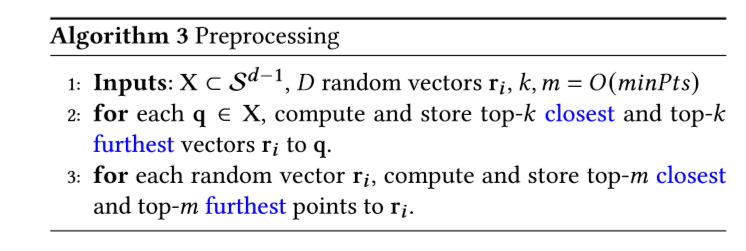
\includegraphics[width=0.7\linewidth]{db-scan-alg3}
	\caption{}
	\label{fig:db-scan-alg3}
	% TODO Replace Screenshot with actual code
\end{figure}

\begin{figure}[h]
	\centering
	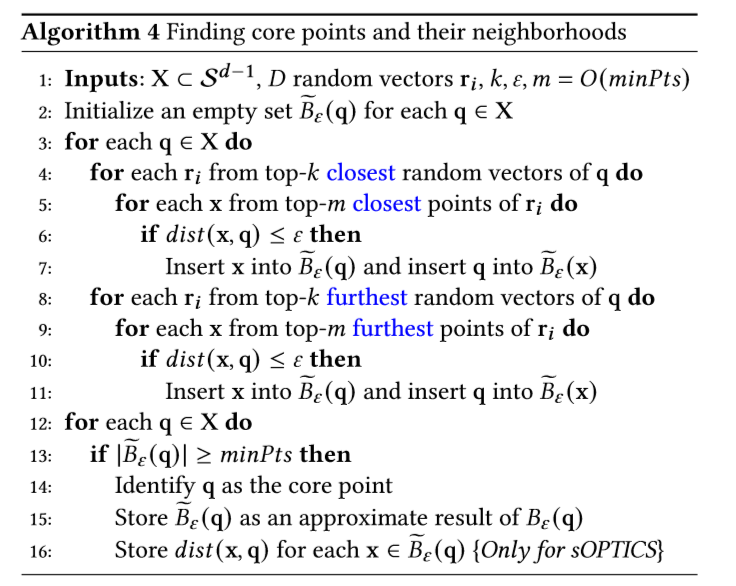
\includegraphics[width=0.7\linewidth]{db-scan-alg4}
	\caption{}
	\label{fig:db-scan-alg4}
	% TODO Replace Screenshot with actual code
\end{figure}

\begin{figure}[h]
	\centering
	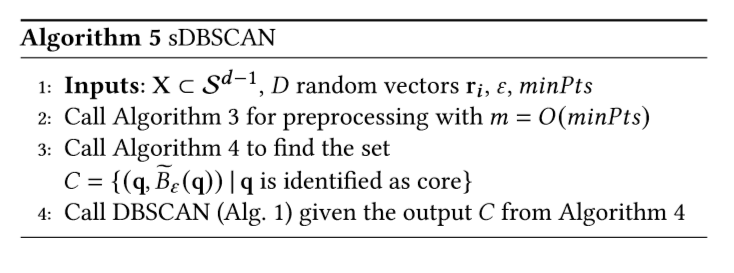
\includegraphics[width=0.7\linewidth]{db-scan-alg5}
	\caption{}
	\label{fig:db-scan-alg5}
	% TODO Replace Screenshot with actual code
\end{figure}


\subsection{GPU Programming with CUDA}

A GPU (Graphical Processing Unit) is based around the idea of having using hundreds to thousands of independent cores to complete tasks in a parallelised manner. This strategy excels in areas such as linear algebra, sorting, and differential equations \cite{Owens2008}. To ease the development of applications that utilize a GPU, NVIDIA, a major manufacturer of GPU chips, has created CUDA \cite{nvidia_cuda} \comment{to provide an API for GPU programming.}{This sentence could be reworded}.

For the purposes of this paper, we will look at the typical architecture of a NVIDIA GPU, then see how this relates to the programming model of CUDA. 

% TODO add note on GPU archicture

The CUDA \comment{programming model}{can it be called a model?} abstracts the low levels of programming directly onto a GPU with a few key concepts. At the highest level there is a \textit{kernel grid}, this executes a single set of instructions called a \textit{kernel} across the GPU. A grid is sub components called \textit{thread blocks} these execute a number of individual kernel instructions - called \textit{threads} - across one SM. A single \textit{thread} is executed on one CUDA core - this is the lowest level of programming abstraction with CUDA. Figure \ref{fig:nvidia-cuda-model} explains these concepts.

\begin{figure}[h]
	\centering
	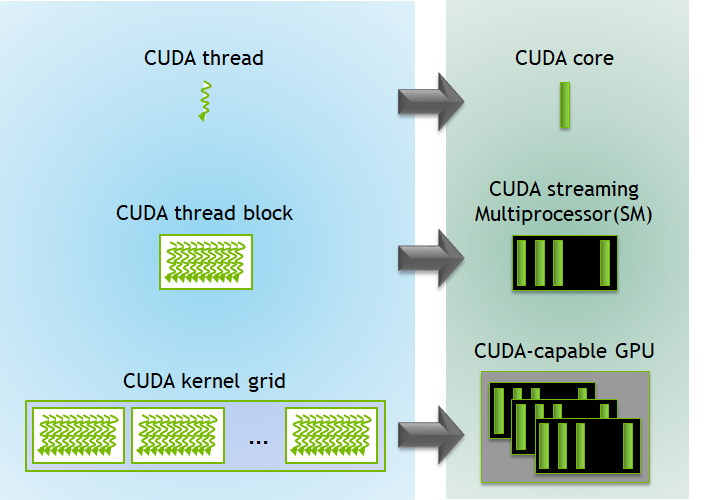
\includegraphics[width=0.7\linewidth]{nvidia-cuda-model}
	\caption{Simplified overview of the CUDA programming model \cite{CUDARefresher2023}}
	\label{fig:nvidia-cuda-model}
\end{figure}


Threads are executed in groups called \textit{warps}. To maximise occupancy of an SM while a block is being executed, the size of a block should be a \comment{multiple of 32}{find a reference for this}.

\section{CUDA-sDBSCAN}

\section{Experiment}

\section{Conclusion}

\bibliographystyle{plain}
\bibliography{refs}

\end{document}
